\begin{center}
\textit{by Martin Bauer, Marcela Carena and Adri\'an Carmona}
\end{center}

In the Two-Higgs-Doublet Model (2HDM), the term $H_1 H_2\equiv H_1^T (i\sigma_2) H_2 $ is a SM singlet which can however be charged under an additional $U(1)$ flavor symmetry. This is an interesting possibility that allows to generate the different fermion masses with a Froggatt-Nielsen (FN) mechanism where the flavon is replaced by the $H_1 H_2$ operator. In this way, the new physics scale $\Lambda$ where the higher dimensional FN operators are generated is tied to the electroweak scale, leading to much stronger phenomenological consequences. Let us assume for concreteness a type-I like 2DHM with the following Yukawa Lagrangian 
\begin{align}
\label{eq:yuk1}
\mathcal{L}_Y&\supset  y^u_{ij} \left(\frac{H_1 H_2}{\Lambda^2}\right)^{n_{u_{ij}}}\bar{q}_L^{i}H_1 u_{R}^j+y^d_{ij} \left(\frac{H_1^{\dagger} H_2^{\dagger}}{\Lambda^2}\right)^{n_{d_{ij}}}\bar{q}_L^{i}\tilde{H}_1 d_{R}^j+y_{ij}^{\ell}\left(\frac{H_1^{\dagger}H_2^{\dagger}}{\Lambda^2}\right)^{n_{e_{ij}}}\bar{\ell}_{L}^i\tilde{H}_1 e_R^j
+\mathrm{h.c.}\,,
\end{align}
where $\tilde{H}_1\equiv i\sigma_2 H^{\ast}_1$ as usual and the charges $n_{u,d,e}$ are a combination of the $U(1)$ charges of $H_1$, $(H_1H_2)$ and the different SM fermion fields. For simplicity, we set the flavor charges of $(H_1 H_2)$ and $H_2$ to $0$ and $1$, respectively, such that  
\begin{align}
n_{u_{ij}}=a_{q_i}-a_{u_j},\quad n_{d_{ij}}=-a_{q_i}+a_{d_j},\quad n_{e_{ij}}=-a_{\ell_i}+a_{e_j},
\end{align}
if we denote by $a_{q_i},a_{u_i}, \ldots,$ the $U(1)$ charges of the SM fermions. In general, the fermion masses are given by
\begin{align}\label{eq:epsilon}
m_\psi=y_{\psi} \varepsilon^{n_\psi} \frac{v}{\sqrt{2}}, \quad \varepsilon = \frac{v_1 v_2}{2\Lambda^2}=\frac{t_\beta}{1+t_\beta^2}\frac{v^2}{2\Lambda^2},
\end{align}
with the vacuum expectation values $\langle H_{1, 2}\rangle=v_{1, 2}$ and $t_\beta \equiv v_1/v_2$. Besides being able to accommodate the observed hierarchy of SM fermion masses and mixing angles for the right assignment of flavor charges \cite{Bauer:2015fxa, Bauer:2015kzy}, this framework can lead to enhanced diagonal Yukawa couplings between the Higgs and the SM fermions while having suppressed flavour changing neutral currents (FCNCs). If we denote by $h$ and $H$ the two neutral scalar mass eigen-states, with $h$ being the observed $125$ \UGeV Higgs, the couplings between the scalars $\varphi=h,H$ and SM fermions $\psi_{L_i, R_i}= P_{L,R} \psi_i$ in the mass eigen-basis read 
\begin{equation}\label{eq:newlagrangian}
\mathcal{L}= g_{\varphi \psi_{L_i} \psi_{R_j} }\, \varphi \,\bar \psi_{L_i} \psi_{R_j}+\mathrm{h.c.}
\end{equation}
with $i$, such that $u_i=u, c,t$,\,  $d_i=d,s,b$ and $e_i=e,\mu,\tau$. This induces 
flavor-diagonal couplings 
\begin{align}\label{eq:diagocoup}
g_{\varphi \psi_{L_i}\psi_{R_i}}= \kappa^\varphi_{\psi_i}\, \frac{m_{\psi_i}}{v} =\left(g^{\varphi}_{\psi_i}(\alpha,\beta)+n_{\psi_i}\, f^\varphi(\alpha, \beta)\right)\frac{m_{\psi_i}}{v},
\end{align}
as well as flavor off-diagonal couplings
 \begin{align}\label{eq:foffc}
g_{\varphi \psi_{L_i}\psi_{R_j}}&=  f^\varphi(\alpha, \beta)\left(\mathcal{A}_{ij}\frac{m_{\psi_j}}{v}-\frac{m_{\psi_i}}{v}\mathcal{B}_{ij} \right)\,.
\end{align}
The flavor universal functions in \eqref{eq:diagocoup} and \eqref{eq:foffc} read
\begin{align}
g^h_{\psi_i}=\frac{c_{\beta-\alpha}}{t_\beta}+s_{\beta-\alpha}\,,\qquad g^H_{\psi_i}=c_{\beta-\alpha}-\frac{s_{\beta-\alpha}}{t_\beta}\,,
\end{align}
and
\begin{align}\label{eq:fFs}
f^h(\alpha,\beta)&=c_{\beta-\alpha}\Big(\frac{1}{t_\beta}-t_\beta\Big)+2s_{\beta-\alpha}\,,\quad f^H(\alpha,\beta)=-s_{\beta-\alpha}\Big(\frac{1}{t_\beta}-t_\beta\Big)+2c_{\beta-\alpha}\,,
\end{align}
where $c_{x}\equiv \cos x$, $s_x\equiv \sin x$. One can see that, unless all flavor charges for a given type of fermions are equal, the off-diagonal elements in matrices $\mathcal{A}$ and $\mathcal{B}$ lead to FCNCs which are chirally suppressed by powers of the ratio~$\varepsilon$, see \cite{Bauer:2017cov} for more details.

The scalar couplings to the different gauge bosons are the same as in a normal type-I 2HDM while the scalar coupling between the heavy Higgs $H$ and two SM Higgs scalars $h$, as well as the triple Higgs coupling can be expressed as \cite{Boudjema:2001ii, Gunion:2002zf}
\begin{align}
\label{eq:mainn1}
g_{Hhh}&=\frac{c_{\beta-\alpha}}{v}\!\left[\big(1\!-\!f^h(\alpha,\beta)s_{\beta-\alpha}\big)\big(3M_A^2\!-\!2m_h^2\!-\!M_H^2\big)\!-\!M_A^2\right],\\
g_{hhh}&= -\frac{3}{v}\!\left[f^h(\alpha,\beta)c_{\beta-\alpha}^2(m_h^2-M_A^2)+m_h^2s_{\beta-\alpha}\right],\label{eq:mainn2}
\end{align}
where $M_A$ is the pseudoscalar mass. The $U(1)$ flavor symmetry restricts the number of allowed terms in the scalar potential forbidding e.g. terms proportional to $H_1 H_2$. The interesting feature is that one can rewrite such self scalar interactions with the help of the function $f^h(\alpha,\beta)$, since it is somehow related to the combination $H_1 H_2^{\dagger}$ appearing in both the scalar potential and the higher dimensional operators generating the different Yukawa couplings. Therefore, the parameter space for which $f^h(\alpha,\beta)\gg 1$ and  $c_{\beta-\alpha}\neq 0$ leads to maximally enhanced diagonal couplings of the SM Higgs to fermions \eqref{eq:diagocoup} as well as to an enhancement of the trilinear couplings \eqref{eq:mainn1} and \eqref{eq:mainn2}. For maximally enhanced Yukawa couplings, the mass of the heavy Higgs $H$ cannot be taken arbitrarily large and resonant Higgs pair production has to be present. This correlation between the enhancement of the Higgs Yukawa couplings $\kappa^h_{\psi}$ and $\text{Br}(H \to hh)$ is illustrated for $M_H=M_A=M_{H^\pm}=500$ \UGeV in Fig. \ref{fig:BRvskappa} where we plot the dependence of $\text{Br}(H \to hh)$ on $c_{\beta-\alpha} $ and $ t_\beta$.  The dashed contours correspond to constant values of $|\kappa_{\psi}^h|$ for $n_{\psi}=1$. This correlation does not dependent of the factor $n_\psi$, although  $n_\psi > 1$ leads to a larger enhancement. The two exceptions for which this correlation breaks down are the limits $c_{\beta-\alpha}\approx 0$ and $c_{\beta-\alpha}\approx \pm 1$. Whereas the second case is strongly disfavoured by SM Higgs couplings strength measurements, the first one (which corresponds to the decoupling limit) is at odds with the flavor model, for it requires large values of the spurion $\mu_3\propto M_A$ which softly breaks the $U(1)$ flavor symmetry. 




%
 \begin{figure}
 \begin{center}
 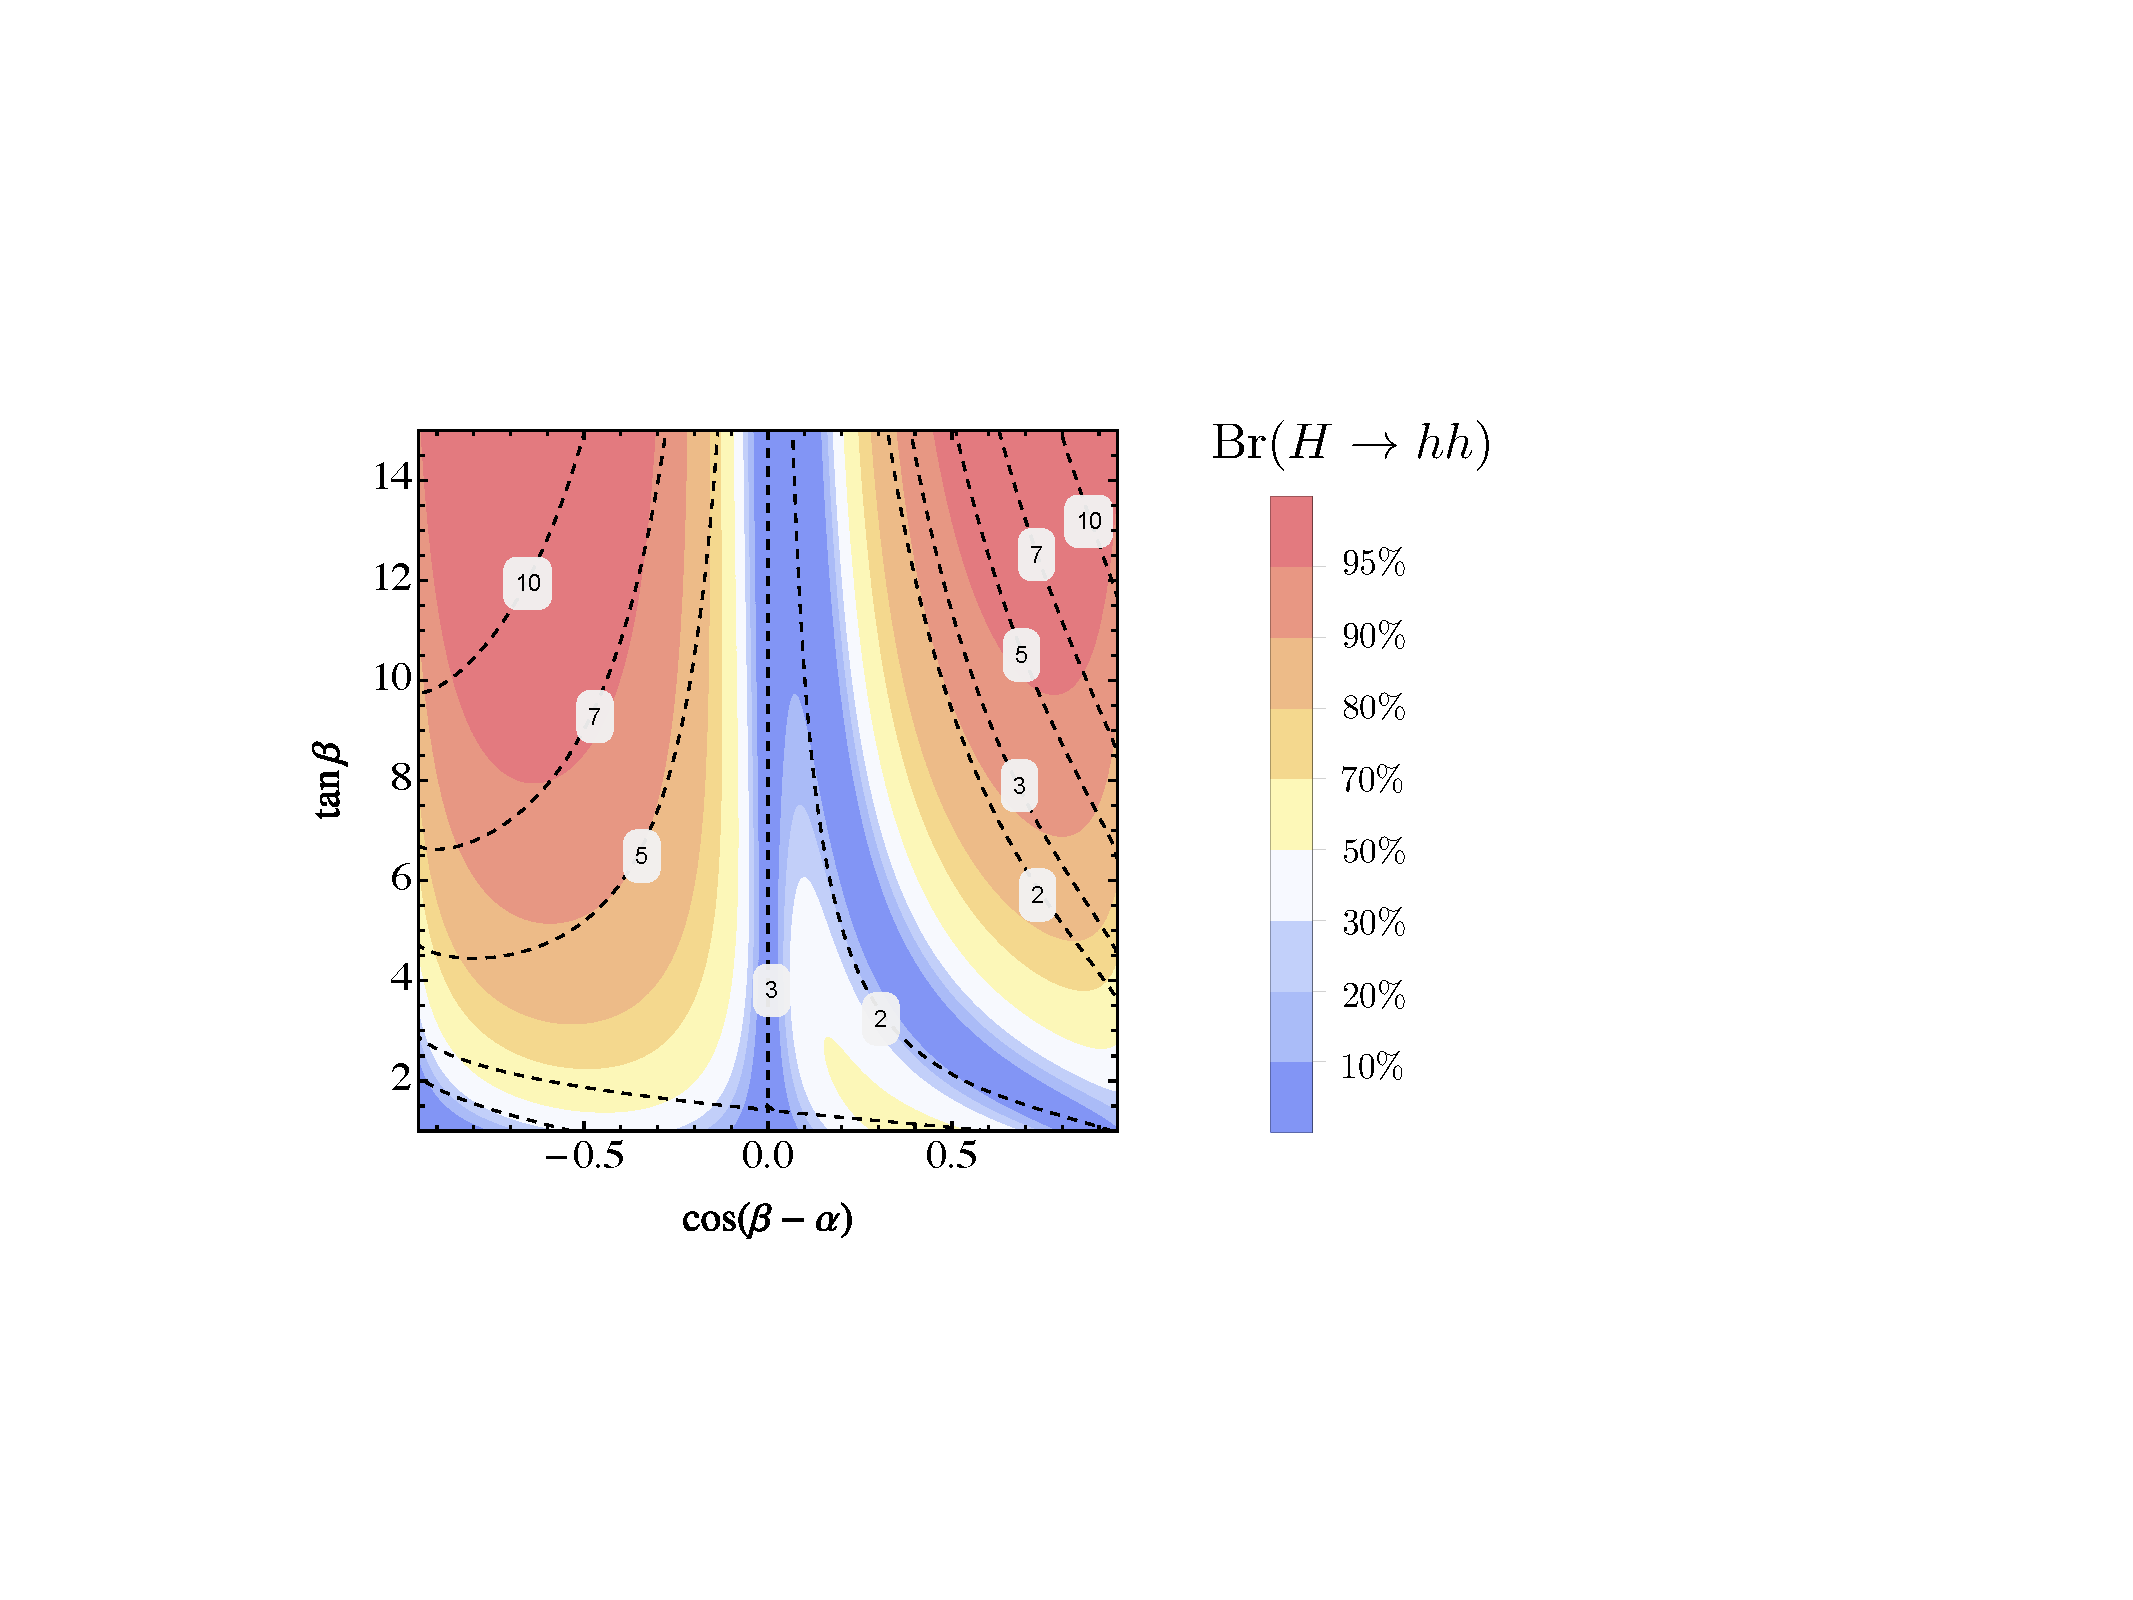
\includegraphics[width=.8\textwidth]{\main/section3/plots/BRvskap.pdf}
 \caption{\label{fig:BRvskappa} $\text{Br}(H \to hh)$ as a function of $\cos(\beta-\alpha)$ and $ \tan\beta$ for $M_H=M_{H^\pm}=550$ \UGeV and $M_A=450$ \UGeV. The dashed contours correspond to constant values $|\kappa_{\psi}^h|$ for $n_{\psi}=1$.}
 \end{center}
  \vspace{-.6cm}
 \end{figure}
%
%
\begin{figure*}
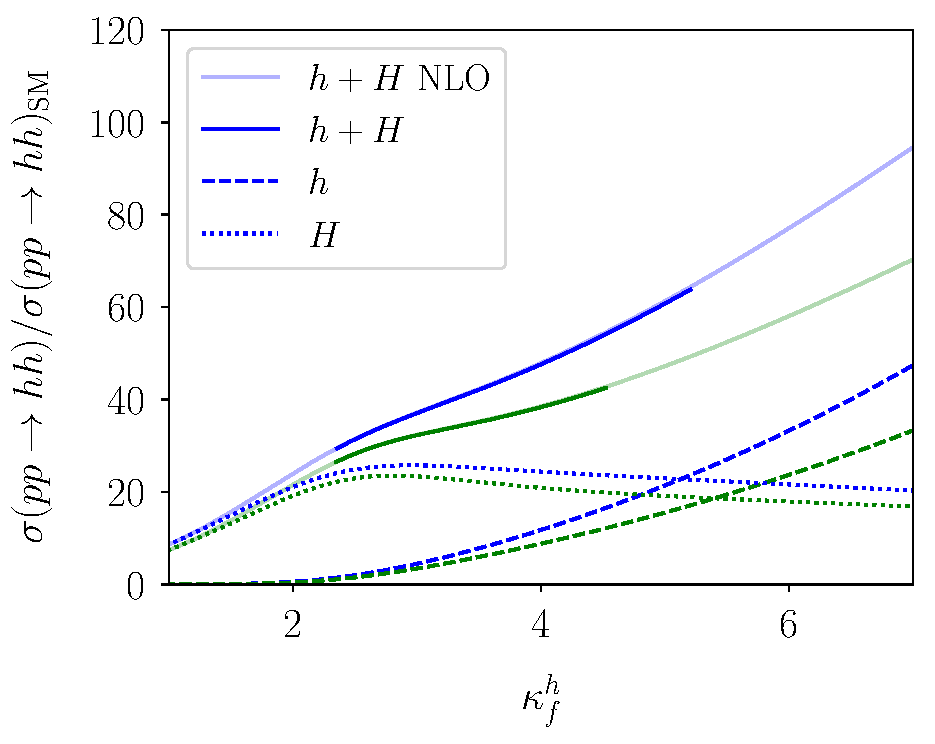
\includegraphics[width=.465\textwidth]{\main/section3/plots/xsec_3.pdf}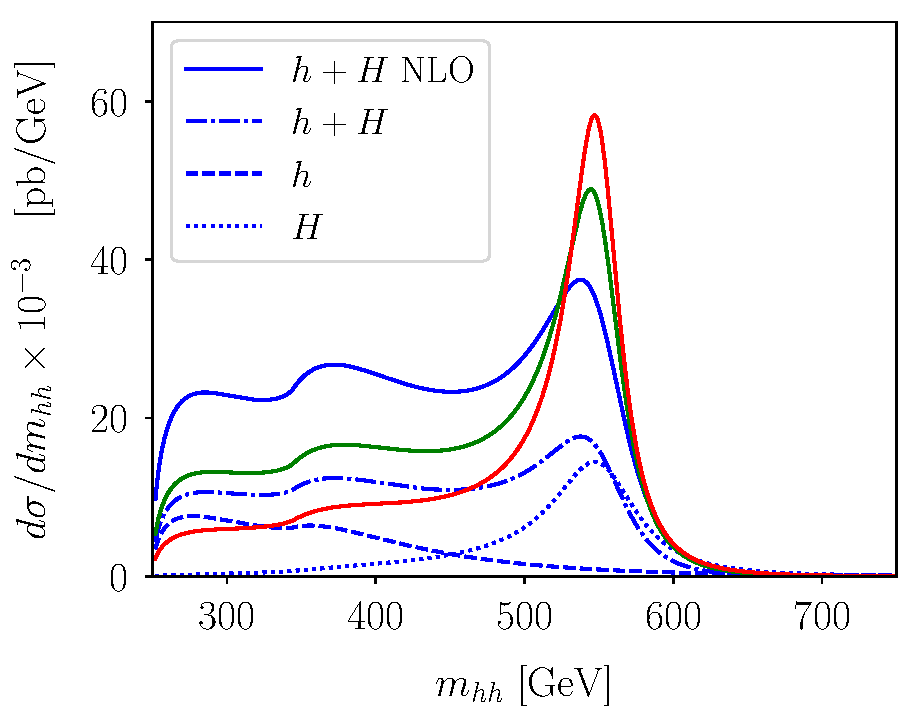
\includegraphics[width=.49\textwidth]{\main/section3/plots/diff.pdf}
	\caption{\label{fig:xsecc} Left: Cross section for Higgs pair production in units of the SM prediction as a function of $\kappa_{\psi}^h$ for $c_{\beta-\alpha}=-0.45~(-0.4)$ and $M_A=450$ \UGeV , $M_H=M_{H^\pm}=550$ \UGeV in blue (green) at $\sqrt{s}=27 $ \UTeV. Right: Invariant mass distribution for the different contributions to the signal with $c_{\beta-\alpha}=-0.45$ and $\kappa^h_{\psi}=5$ (blue),  $\kappa_{\psi}^h=4$ (green) and $\kappa_{\psi}^h=3$ (red) at $\sqrt{s}=27 $ \UTeV, respectively.} 
	\label{fig:hhflavourxsanddistr}
\end{figure*}
%

The enhancement in $\text{Br}(H\to hh)$ shown in Figure~\ref{fig:BRvskappa} is partially cancelled in the production cross section $\sigma(gg\to H)$ for large values of $t_{\beta}$ due to the fact that $\sigma(gg\to H)\propto 1+1/t_\beta^2-(\kappa_t^h)^2$, with $\kappa_t^h \approx 1$. However, the cross-section $\sigma(gg\to h\to hh)$ is not suppressed for such values of $t_{\beta}$ and the combination of both contributions leads to a continuous enhancement in the di-Higgs cross-section. There is therefore a non-trivial interplay between resonant and non-resonant contributions, which we illustrate in the left panel of Fig.~\ref{fig:xsecc}, where we plot both contributions assuming as a function of $\kappa_{\psi}^h$ for fixed values of $c_{\beta-\alpha}$ (which is a monotonic function of $t_{\beta}$). We assume a centre-of-mass energy of $\sqrt{s}=27$ \UTeV and set $M_A=450$ \UGeV and $M_{H}=M_{H^{\pm}}=550$ \UGeV, while choosing two different values of $c_{\beta-\alpha}=-0.45$ and $-0.4$. Dashed (dotted) lines correspond to the non-resonant (resonant) contributions, whereas the solid lines represent the full $\sigma(gg\to hh)$ in the 2HDM in units of the SM prediction, both at LO and NLO.   Solid lines show the NLO results, while the solid shaded lines mark the values of $\kappa_{\psi}$ excluded by perturbativity and unitarity constraints~\cite{Eriksson:2009ws}.  More details about the calculation of the signal and plots for $\sqrt{s}=13$ \UTeV can be found in Ref.~\cite{Bauer:2017cov}.  The values of $\kappa_{\psi}^h$ in Fig.~\ref{fig:xsecc} correspond to $n_{\psi}=1$ but values of $\mathcal{O}(10)$ and larger are obtained for $n_{\psi}>1$. We also show in the right panel of Fig.~\ref{fig:xsecc} the invariant mass distribution for the different contributions to the di-Higgs signal for $c_{\beta-\alpha}=-0.45$ and three different values of $\kappa_{\psi}^{h}=3, 4$ and $5$. The interesting feature is that, when the enhancement in the Higgs Yukawa couplings is large enough, the interference between both non-resonant and resonant contributions turns the broad peak into a shoulder in the $d\sigma/ dm_{hh}$ distribution for the total cross section, as shown for the case $\kappa_{\psi}^h=5$ by the blue line in the right panel of Fig.~\ref{fig:xsecc}. Resolving such shape in the  invariant mass distribution can be quite challenging. We encourage a dedicated analysis considering the corresponding $d\sigma/dm_{hh}$ templates to maximise the sensitivity to features in the di-Higgs invariant mass distribution from the simultaneous enhancement of  $g_{hhh}$, $g_{Hhh}$ and $\kappa^h_{\psi}$.\\

